\documentclass[11pt]{article}

% load some asm stuff -
\usepackage{amssymb}
\usepackage{amsmath}
\usepackage{amsthm}
%\usepackage{palatino,lettrine}
\usepackage{fancyhdr}
\usepackage{epsfig}
\usepackage[square,sort,comma,numbers]{natbib}
\usepackage{simplemargins}
\usepackage{setspace}
\usepackage{wrapfig}
\usepackage{hyperref}
%\usepackage{boiboites}
\usepackage[margin=0pt,font=small,labelfont=bf]{caption}
\newcommand{\boldindex}[1]{\textbf{\hyperpage{#1}}}
\usepackage{makeidx}\makeindex
\bibliographystyle{plos2015}

\usepackage{algpseudocode}
\usepackage{algorithm}


% Set the size
%\textwidth = 6.75 in
%\textheight = 9.75 in
%\oddsidemargin = 0.0 in
%\evensidemargin = 0.0 in
%\topmargin = 0.01 in
%\headheight = 0.0 in
%\headsep = 0.25 in
%\parskip = 0.15in
% \doublespace
\setallmargins{1in}

\newtheorem{example}{Example}[section]
\newtheorem{thm}{Theorem}[section]
\newtheorem{property}{Property}[section]

\theoremstyle{definition}
\newtheorem{defn}[thm]{Definition}

\makeatletter
% \renewcommand\subsection{\@startsection
% 	{subsection}{2}{0mm}
% 	{-0.05in}
% 	{0.05\baselineskip}
% 	{\normalfont\normalsize\bfseries}}
\renewcommand\subsubsection{\@startsection
	{subsubsection}{2}{0mm}
	{-0.05in}
	{-0.5\baselineskip}
	{\normalfont\normalsize\itshape\bfseries}}
\renewcommand\paragraph{\@startsection
	{paragraph}{2}{0mm}
	{-0.05in}
	{-0.5\baselineskip}
	{\normalfont\normalsize\itshape}}
\makeatother
\linespread{1.1}

\fancypagestyle{proposal}{\fancyhf{}%
	\fancyhead[RO,LE]{\thepage}%
	\fancyhead[LO,RE]{CHEME 133 Module 2 American Call Contracts at Expiration}%
	\renewcommand\headrulewidth{1pt}}
\pagestyle{proposal}

\usepackage{mdframed}
\definecolor{lgray}{rgb}{0.92,0.92,0.92}
\definecolor{antiquewhite}{rgb}{0.98,0.92,0.84}
\definecolor{lightskyblue}{rgb}{0.93,0.95,0.99}

% defn environment
\mdfdefinestyle{theoremstyle}{% 
    linecolor=black,linewidth=1pt,% 
    frametitlerule=true,% 
    frametitlebackgroundcolor=lgray, 
    innertopmargin=\topskip,} 
\mdtheorem[style=theoremstyle]{definition}{Definition}

% concept environment
\mdfdefinestyle{conceptstyle}{% 
    linecolor=black,linewidth=1pt,% 
    frametitlerule=true,% 
    frametitlebackgroundcolor=lightskyblue, 
    innertopmargin=\topskip,} 
\mdtheorem[style=conceptstyle]{concept}{Concept}
\newcommand{\newterm}[1]{{\it #1}}

% Single space'd bib -
\setlength\bibsep{0pt}

\renewcommand{\rmdefault}{phv}\renewcommand{\sfdefault}{phv}
%\newboxedtheorem[boxcolor=black, background=gray!5,titlebackground=orange!20,titleboxcolor = black]{color_box_example}{Example}{test}

% Change the number format in the ref list -
\renewcommand{\bibnumfmt}[1]{#1.}

% Change Figure to Fig.
\renewcommand{\figurename}{Fig.}
\usepackage{enumitem}
\setlist{noitemsep} % or \setlist{noitemsep} to leave space around whole list

%Joycelyn Chan, Joshua Lequieu, Michael Paull, Chidanand Balaji, Ryan Tasseff
%Our derivation follows closely the earlier development of Fredrickson \citep{Fredrickson:1976fk}.

% Begin ...
\begin{document}

%\begin{titlepage}
{\par\centering\textbf{\Large CHEME 133 Module 2: Introduction to American Style Call Contracts at Expiration}}
\vspace{0.2in}
{\par \centering \large{Jeffrey D. Varner}}
\vspace{0.05in}
{\par \centering \large{Smith School of Chemical and Biomolecular Engineering}}
{\par \centering \large{Cornell University, Ithaca NY 14853}}
% \vspace{0.1in}
% {\par \centering \small{Copyright \copyright\ Jeffrey Varner 2018. All Rights Reserved.}}\\

%\end{titlepage}
\date{}
\thispagestyle{empty}

\setcounter{page}{1}

\section*{Introduction}
A \texttt{call} contract gives the holder (buyer) the right, but not the obligation, to purchase a specified asset, 
such as stocks, commodities, or currencies, to their counterparty (contract seller). 
Let's consider stock as the underlying asset. A single standard options contract controls 100 shares of stock. 
From the buyer's perspective, call contracts allow an investor to benefit from upside price movement of a stock without purchasing the stock.
Further, call options (again from the buyer's perspective) have limited downside risk, i.e., the maximum amount that the holder of the call option can lose 
is the premium paid for the option. Finally, call options are a mechanism to purchase shares of stock at the strike price of $K$ instead of the market price of $S$. 
On other hand, from the seller's perspective, the main objective of selling a call contract is to collect the premium $\mathcal{P}$. 
Call contracts also allow the seller to benefit from downward price movement without purchasing shares of stock (in the case of a naked call).
However, for a seller, call options have unlimted upside risk; 
Thus, call options are often only sold by investors who already own the required number of shares of stock 
(known as a \href{https://www.investopedia.com/terms/c/coveredcall.asp}{covered call position}. 

\begin{concept}[Americam versus European Call Contracts]
The key difference between an American and European call contracts is the time at which the option can be exercised.
An American call contract can be exercised at any time on or before the expiration date, while a European call contract can only be exercised at expiration.
The extra flexibility of an American call contract comes at a cost, and thus the premium for an American call contract is at least that of a European call contract.
\end{concept}

\section*{American Call Options}
The payoff per share at expiration for a call option is:
\begin{equation*}
V_{c}(K,S(T)) = \max\left(S(T) - K,~0\right)
\end{equation*}
where $K$ denotes the strike price and $S(T)$ is the share price at expiration. 
The \texttt{seller} charges the \texttt{buyer} a premium $\mathcal{P}_{c}(K,S(0))$ for each contract.
The buyer's profit per share at expiration is the payoff minus the contract premium:
\begin{equation*}
P_{c}(K,S(T)) = V_{c}(K,S(T)) -  \mathcal{P}_{c}(K,S(0))
\end{equation*}
The premium (cost) for each contract is governed by:
\begin{equation*}
\mathcal{P}_{c}(K,S(0))\geq\mathbb{E}\Bigl(\mathcal{D}^{-1}_{T,0}(\bar{r})\cdot{V_{c}}(K,S(T))\Bigr)
\end{equation*}
where $\mathcal{D}_{T,0}(\bar{r})$ denotes the risk neutral discount factor computed between purchase and contract expiration.

\begin{figure}[ht]
    \centering
    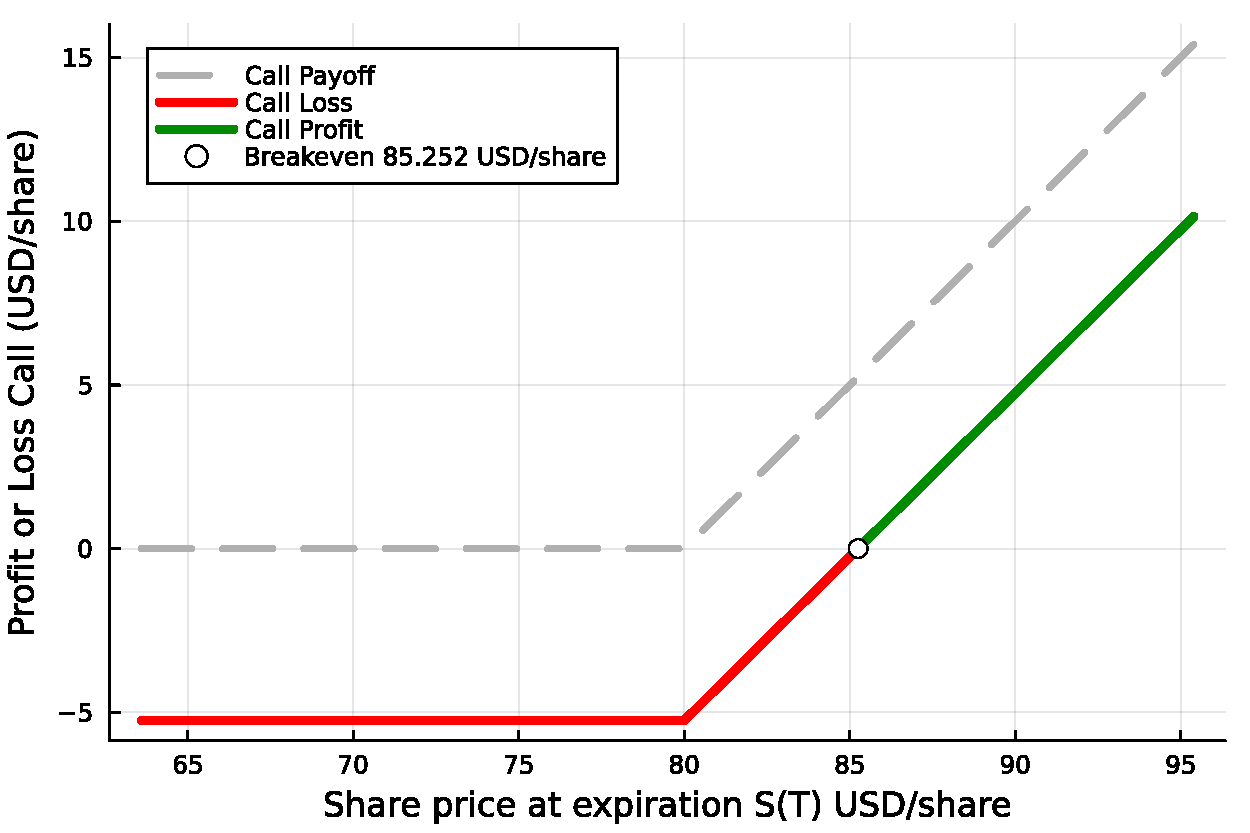
\includegraphics[width=0.65\textwidth]{./figs/Fig-Example-Call-K80-62DTE.pdf}
    \caption{Schematic of the payoff, profit and breakeven for a \texttt{long call} 
	contract. The gray dashed line denotes the payoff at expiration for the buyer.
	The red line denotes share prices at expiration that result in a loss for the buyer, 
	while the green line denotes share prices at expiration that result in a profit for the buyer.
	Parameters: the \texttt{call} 
	contract strike price is $K$ = 80 USD/share and the premium $\mathcal{P}_{c}$ = 5.25 USD/share.}\label{fig:call-payoff-profit-breakeven-diagram}
\end{figure}

\section*{Summary}
In this module we introduced American style call contracts.
A \texttt{call} contract gives the holder the right, but not the obligation, to buy an underlying asset at a specified price (strike) on or before a future date (expiration).
We introduced the payoff and profit diagrams for \texttt{call} contracts.

% \bibliography{References_v1}

\clearpage
\printindex

\end{document}
